% Options for packages loaded elsewhere
% Options for packages loaded elsewhere
\PassOptionsToPackage{unicode}{hyperref}
\PassOptionsToPackage{hyphens}{url}
\PassOptionsToPackage{dvipsnames,svgnames,x11names}{xcolor}
%
\documentclass[
  letterpaper,
  DIV=11,
  numbers=noendperiod]{scrartcl}
\usepackage{xcolor}
\usepackage{amsmath,amssymb}
\setcounter{secnumdepth}{-\maxdimen} % remove section numbering
\usepackage{iftex}
\ifPDFTeX
  \usepackage[T1]{fontenc}
  \usepackage[utf8]{inputenc}
  \usepackage{textcomp} % provide euro and other symbols
\else % if luatex or xetex
  \usepackage{unicode-math} % this also loads fontspec
  \defaultfontfeatures{Scale=MatchLowercase}
  \defaultfontfeatures[\rmfamily]{Ligatures=TeX,Scale=1}
\fi
\usepackage{lmodern}
\ifPDFTeX\else
  % xetex/luatex font selection
\fi
% Use upquote if available, for straight quotes in verbatim environments
\IfFileExists{upquote.sty}{\usepackage{upquote}}{}
\IfFileExists{microtype.sty}{% use microtype if available
  \usepackage[]{microtype}
  \UseMicrotypeSet[protrusion]{basicmath} % disable protrusion for tt fonts
}{}
\makeatletter
\@ifundefined{KOMAClassName}{% if non-KOMA class
  \IfFileExists{parskip.sty}{%
    \usepackage{parskip}
  }{% else
    \setlength{\parindent}{0pt}
    \setlength{\parskip}{6pt plus 2pt minus 1pt}}
}{% if KOMA class
  \KOMAoptions{parskip=half}}
\makeatother
% Make \paragraph and \subparagraph free-standing
\makeatletter
\ifx\paragraph\undefined\else
  \let\oldparagraph\paragraph
  \renewcommand{\paragraph}{
    \@ifstar
      \xxxParagraphStar
      \xxxParagraphNoStar
  }
  \newcommand{\xxxParagraphStar}[1]{\oldparagraph*{#1}\mbox{}}
  \newcommand{\xxxParagraphNoStar}[1]{\oldparagraph{#1}\mbox{}}
\fi
\ifx\subparagraph\undefined\else
  \let\oldsubparagraph\subparagraph
  \renewcommand{\subparagraph}{
    \@ifstar
      \xxxSubParagraphStar
      \xxxSubParagraphNoStar
  }
  \newcommand{\xxxSubParagraphStar}[1]{\oldsubparagraph*{#1}\mbox{}}
  \newcommand{\xxxSubParagraphNoStar}[1]{\oldsubparagraph{#1}\mbox{}}
\fi
\makeatother

\usepackage{color}
\usepackage{fancyvrb}
\newcommand{\VerbBar}{|}
\newcommand{\VERB}{\Verb[commandchars=\\\{\}]}
\DefineVerbatimEnvironment{Highlighting}{Verbatim}{commandchars=\\\{\}}
% Add ',fontsize=\small' for more characters per line
\usepackage{framed}
\definecolor{shadecolor}{RGB}{241,243,245}
\newenvironment{Shaded}{\begin{snugshade}}{\end{snugshade}}
\newcommand{\AlertTok}[1]{\textcolor[rgb]{0.68,0.00,0.00}{#1}}
\newcommand{\AnnotationTok}[1]{\textcolor[rgb]{0.37,0.37,0.37}{#1}}
\newcommand{\AttributeTok}[1]{\textcolor[rgb]{0.40,0.45,0.13}{#1}}
\newcommand{\BaseNTok}[1]{\textcolor[rgb]{0.68,0.00,0.00}{#1}}
\newcommand{\BuiltInTok}[1]{\textcolor[rgb]{0.00,0.23,0.31}{#1}}
\newcommand{\CharTok}[1]{\textcolor[rgb]{0.13,0.47,0.30}{#1}}
\newcommand{\CommentTok}[1]{\textcolor[rgb]{0.37,0.37,0.37}{#1}}
\newcommand{\CommentVarTok}[1]{\textcolor[rgb]{0.37,0.37,0.37}{\textit{#1}}}
\newcommand{\ConstantTok}[1]{\textcolor[rgb]{0.56,0.35,0.01}{#1}}
\newcommand{\ControlFlowTok}[1]{\textcolor[rgb]{0.00,0.23,0.31}{\textbf{#1}}}
\newcommand{\DataTypeTok}[1]{\textcolor[rgb]{0.68,0.00,0.00}{#1}}
\newcommand{\DecValTok}[1]{\textcolor[rgb]{0.68,0.00,0.00}{#1}}
\newcommand{\DocumentationTok}[1]{\textcolor[rgb]{0.37,0.37,0.37}{\textit{#1}}}
\newcommand{\ErrorTok}[1]{\textcolor[rgb]{0.68,0.00,0.00}{#1}}
\newcommand{\ExtensionTok}[1]{\textcolor[rgb]{0.00,0.23,0.31}{#1}}
\newcommand{\FloatTok}[1]{\textcolor[rgb]{0.68,0.00,0.00}{#1}}
\newcommand{\FunctionTok}[1]{\textcolor[rgb]{0.28,0.35,0.67}{#1}}
\newcommand{\ImportTok}[1]{\textcolor[rgb]{0.00,0.46,0.62}{#1}}
\newcommand{\InformationTok}[1]{\textcolor[rgb]{0.37,0.37,0.37}{#1}}
\newcommand{\KeywordTok}[1]{\textcolor[rgb]{0.00,0.23,0.31}{\textbf{#1}}}
\newcommand{\NormalTok}[1]{\textcolor[rgb]{0.00,0.23,0.31}{#1}}
\newcommand{\OperatorTok}[1]{\textcolor[rgb]{0.37,0.37,0.37}{#1}}
\newcommand{\OtherTok}[1]{\textcolor[rgb]{0.00,0.23,0.31}{#1}}
\newcommand{\PreprocessorTok}[1]{\textcolor[rgb]{0.68,0.00,0.00}{#1}}
\newcommand{\RegionMarkerTok}[1]{\textcolor[rgb]{0.00,0.23,0.31}{#1}}
\newcommand{\SpecialCharTok}[1]{\textcolor[rgb]{0.37,0.37,0.37}{#1}}
\newcommand{\SpecialStringTok}[1]{\textcolor[rgb]{0.13,0.47,0.30}{#1}}
\newcommand{\StringTok}[1]{\textcolor[rgb]{0.13,0.47,0.30}{#1}}
\newcommand{\VariableTok}[1]{\textcolor[rgb]{0.07,0.07,0.07}{#1}}
\newcommand{\VerbatimStringTok}[1]{\textcolor[rgb]{0.13,0.47,0.30}{#1}}
\newcommand{\WarningTok}[1]{\textcolor[rgb]{0.37,0.37,0.37}{\textit{#1}}}

\usepackage{longtable,booktabs,array}
\usepackage{calc} % for calculating minipage widths
% Correct order of tables after \paragraph or \subparagraph
\usepackage{etoolbox}
\makeatletter
\patchcmd\longtable{\par}{\if@noskipsec\mbox{}\fi\par}{}{}
\makeatother
% Allow footnotes in longtable head/foot
\IfFileExists{footnotehyper.sty}{\usepackage{footnotehyper}}{\usepackage{footnote}}
\makesavenoteenv{longtable}
\usepackage{graphicx}
\makeatletter
\newsavebox\pandoc@box
\newcommand*\pandocbounded[1]{% scales image to fit in text height/width
  \sbox\pandoc@box{#1}%
  \Gscale@div\@tempa{\textheight}{\dimexpr\ht\pandoc@box+\dp\pandoc@box\relax}%
  \Gscale@div\@tempb{\linewidth}{\wd\pandoc@box}%
  \ifdim\@tempb\p@<\@tempa\p@\let\@tempa\@tempb\fi% select the smaller of both
  \ifdim\@tempa\p@<\p@\scalebox{\@tempa}{\usebox\pandoc@box}%
  \else\usebox{\pandoc@box}%
  \fi%
}
% Set default figure placement to htbp
\def\fps@figure{htbp}
\makeatother





\setlength{\emergencystretch}{3em} % prevent overfull lines

\providecommand{\tightlist}{%
  \setlength{\itemsep}{0pt}\setlength{\parskip}{0pt}}



 


\KOMAoption{captions}{tableheading}
\makeatletter
\@ifpackageloaded{caption}{}{\usepackage{caption}}
\AtBeginDocument{%
\ifdefined\contentsname
  \renewcommand*\contentsname{Table of contents}
\else
  \newcommand\contentsname{Table of contents}
\fi
\ifdefined\listfigurename
  \renewcommand*\listfigurename{List of Figures}
\else
  \newcommand\listfigurename{List of Figures}
\fi
\ifdefined\listtablename
  \renewcommand*\listtablename{List of Tables}
\else
  \newcommand\listtablename{List of Tables}
\fi
\ifdefined\figurename
  \renewcommand*\figurename{Figure}
\else
  \newcommand\figurename{Figure}
\fi
\ifdefined\tablename
  \renewcommand*\tablename{Table}
\else
  \newcommand\tablename{Table}
\fi
}
\@ifpackageloaded{float}{}{\usepackage{float}}
\floatstyle{ruled}
\@ifundefined{c@chapter}{\newfloat{codelisting}{h}{lop}}{\newfloat{codelisting}{h}{lop}[chapter]}
\floatname{codelisting}{Listing}
\newcommand*\listoflistings{\listof{codelisting}{List of Listings}}
\makeatother
\makeatletter
\makeatother
\makeatletter
\@ifpackageloaded{caption}{}{\usepackage{caption}}
\@ifpackageloaded{subcaption}{}{\usepackage{subcaption}}
\makeatother
\usepackage{bookmark}
\IfFileExists{xurl.sty}{\usepackage{xurl}}{} % add URL line breaks if available
\urlstyle{same}
\hypersetup{
  pdftitle={Decision Tree Challenge},
  colorlinks=true,
  linkcolor={blue},
  filecolor={Maroon},
  citecolor={Blue},
  urlcolor={Blue},
  pdfcreator={LaTeX via pandoc}}


\title{Decision Tree Challenge}
\usepackage{etoolbox}
\makeatletter
\providecommand{\subtitle}[1]{% add subtitle to \maketitle
  \apptocmd{\@title}{\par {\large #1 \par}}{}{}
}
\makeatother
\subtitle{Feature Importance and Categorical Variable Encoding}
\author{}
\date{}
\begin{document}
\maketitle


\section{🌳 Decision Tree Challenge - Feature Importance and Variable
Encoding}\label{decision-tree-challenge---feature-importance-and-variable-encoding}

\subsection{The Decision Tree Problem
🎯}\label{the-decision-tree-problem}

Decision trees can be helpful when searching for analysis that has
interpretability and versitility. However, flaws occur when we mark
categorical variables as numbers. Decision trees react as if the
sequence of numbers have a meaning, which can jumble the transparency of
our analysis. This is why feature importance is established. Feature
importance measures the amount that each variable contributes to the
improvement of prediction accuracy. This applies for all splits in the
tree. This is the path to understanding which variables have the
greatest significance as predictors.

\subsubsection{R}\label{r}

\begin{Shaded}
\begin{Highlighting}[]
\CommentTok{\# Load libraries}
\FunctionTok{suppressPackageStartupMessages}\NormalTok{(}\FunctionTok{library}\NormalTok{(tidyverse))}
\FunctionTok{suppressPackageStartupMessages}\NormalTok{(}\FunctionTok{library}\NormalTok{(rpart))}
\ControlFlowTok{if}\NormalTok{ (}\SpecialCharTok{!}\FunctionTok{require}\NormalTok{(rpart.plot, }\AttributeTok{quietly =} \ConstantTok{TRUE}\NormalTok{)) \{}
  \FunctionTok{install.packages}\NormalTok{(}\StringTok{"rpart.plot"}\NormalTok{, }\AttributeTok{repos =} \StringTok{"https://cran.rstudio.com/"}\NormalTok{)}
  \FunctionTok{library}\NormalTok{(rpart.plot)}
\NormalTok{\}}

\CommentTok{\# Load data}
\NormalTok{sales\_data }\OtherTok{\textless{}{-}} \FunctionTok{read.csv}\NormalTok{(}\StringTok{"https://raw.githubusercontent.com/flyaflya/buad442Fall2025/refs/heads/main/datasets/salesPriceData.csv"}\NormalTok{)}

\CommentTok{\# Prepare model data (treating zipCode as numerical)}
\NormalTok{model\_data }\OtherTok{\textless{}{-}}\NormalTok{ sales\_data }\SpecialCharTok{\%\textgreater{}\%}
  \FunctionTok{select}\NormalTok{(SalePrice, LotArea, YearBuilt, GrLivArea, FullBath, HalfBath, }
\NormalTok{         BedroomAbvGr, TotRmsAbvGrd, GarageCars, zipCode) }\SpecialCharTok{\%\textgreater{}\%}
  \FunctionTok{na.omit}\NormalTok{()}

\CommentTok{\# Split data}
\FunctionTok{set.seed}\NormalTok{(}\DecValTok{123}\NormalTok{)}
\NormalTok{train\_indices }\OtherTok{\textless{}{-}} \FunctionTok{sample}\NormalTok{(}\DecValTok{1}\SpecialCharTok{:}\FunctionTok{nrow}\NormalTok{(model\_data), }\FloatTok{0.8} \SpecialCharTok{*} \FunctionTok{nrow}\NormalTok{(model\_data))}
\NormalTok{train\_data }\OtherTok{\textless{}{-}}\NormalTok{ model\_data[train\_indices, ]}
\NormalTok{test\_data }\OtherTok{\textless{}{-}}\NormalTok{ model\_data[}\SpecialCharTok{{-}}\NormalTok{train\_indices, ]}

\CommentTok{\# Build decision tree}
\NormalTok{tree\_model }\OtherTok{\textless{}{-}} \FunctionTok{rpart}\NormalTok{(SalePrice }\SpecialCharTok{\textasciitilde{}}\NormalTok{ ., }
                    \AttributeTok{data =}\NormalTok{ train\_data,}
                    \AttributeTok{method =} \StringTok{"anova"}\NormalTok{,}
                    \AttributeTok{control =} \FunctionTok{rpart.control}\NormalTok{(}\AttributeTok{maxdepth =} \DecValTok{3}\NormalTok{, }
                                          \AttributeTok{minsplit =} \DecValTok{20}\NormalTok{, }
                                          \AttributeTok{minbucket =} \DecValTok{10}\NormalTok{))}

\FunctionTok{cat}\NormalTok{(}\StringTok{"Model built with"}\NormalTok{, }\FunctionTok{sum}\NormalTok{(tree\_model}\SpecialCharTok{$}\NormalTok{frame}\SpecialCharTok{$}\NormalTok{var }\SpecialCharTok{==} \StringTok{"\textless{}leaf\textgreater{}"}\NormalTok{), }\StringTok{"terminal nodes}\SpecialCharTok{\textbackslash{}n}\StringTok{"}\NormalTok{)}
\end{Highlighting}
\end{Shaded}

\begin{verbatim}
Model built with 7 terminal nodes
\end{verbatim}

\subsection{Tree Visualization}\label{tree-visualization}

\subsubsection{R}\label{r-1}

\begin{Shaded}
\begin{Highlighting}[]
\CommentTok{\# Visualize tree}
\ControlFlowTok{if}\NormalTok{ (}\FunctionTok{require}\NormalTok{(rpart.plot, }\AttributeTok{quietly =} \ConstantTok{TRUE}\NormalTok{)) \{}
  \FunctionTok{rpart.plot}\NormalTok{(tree\_model, }
             \AttributeTok{type =} \DecValTok{2}\NormalTok{,}
             \AttributeTok{extra =} \DecValTok{101}\NormalTok{,}
             \AttributeTok{fallen.leaves =} \ConstantTok{TRUE}\NormalTok{,}
             \AttributeTok{digits =} \DecValTok{0}\NormalTok{,}
             \AttributeTok{cex =} \FloatTok{0.8}\NormalTok{,}
             \AttributeTok{main =} \StringTok{"Decision Tree (zipCode as Numerical)"}\NormalTok{)}
\NormalTok{\} }\ControlFlowTok{else}\NormalTok{ \{}
  \FunctionTok{plot}\NormalTok{(tree\_model, }\AttributeTok{uniform =} \ConstantTok{TRUE}\NormalTok{, }\AttributeTok{main =} \StringTok{"Decision Tree (zipCode as Numerical)"}\NormalTok{)}
  \FunctionTok{text}\NormalTok{(tree\_model, }\AttributeTok{use.n =} \ConstantTok{TRUE}\NormalTok{, }\AttributeTok{all =} \ConstantTok{TRUE}\NormalTok{, }\AttributeTok{cex =} \FloatTok{0.8}\NormalTok{)}
\NormalTok{\}}
\end{Highlighting}
\end{Shaded}

\pandocbounded{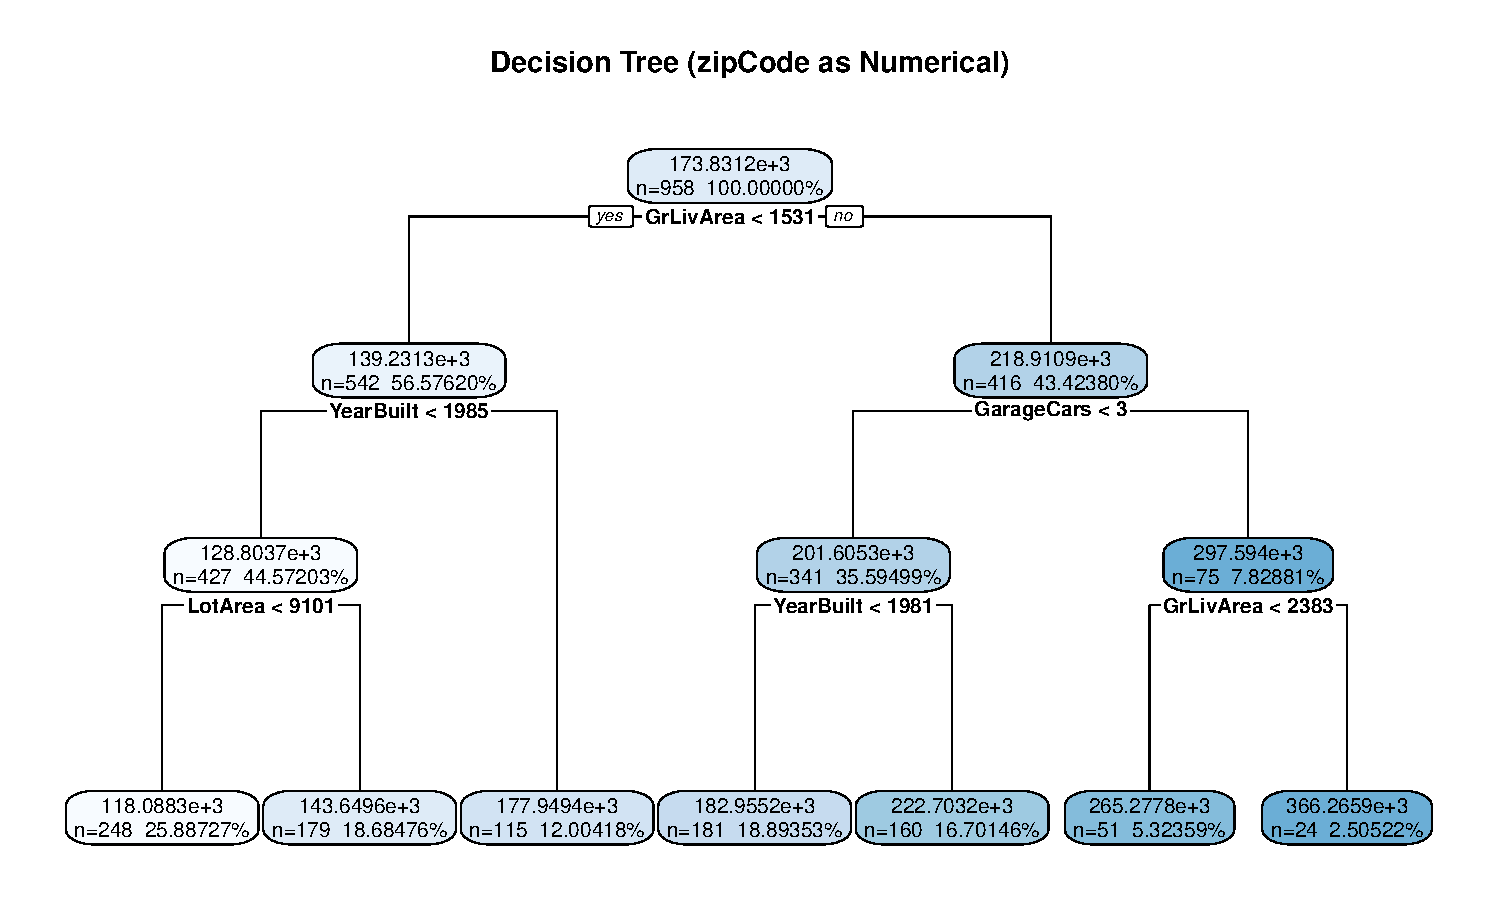
\includegraphics[keepaspectratio]{index_files/figure-pdf/visualize-tree-r-1.pdf}}

\subsection{Feature Importance
Analysis}\label{feature-importance-analysis}

\subsubsection{R}\label{r-2}

\pandocbounded{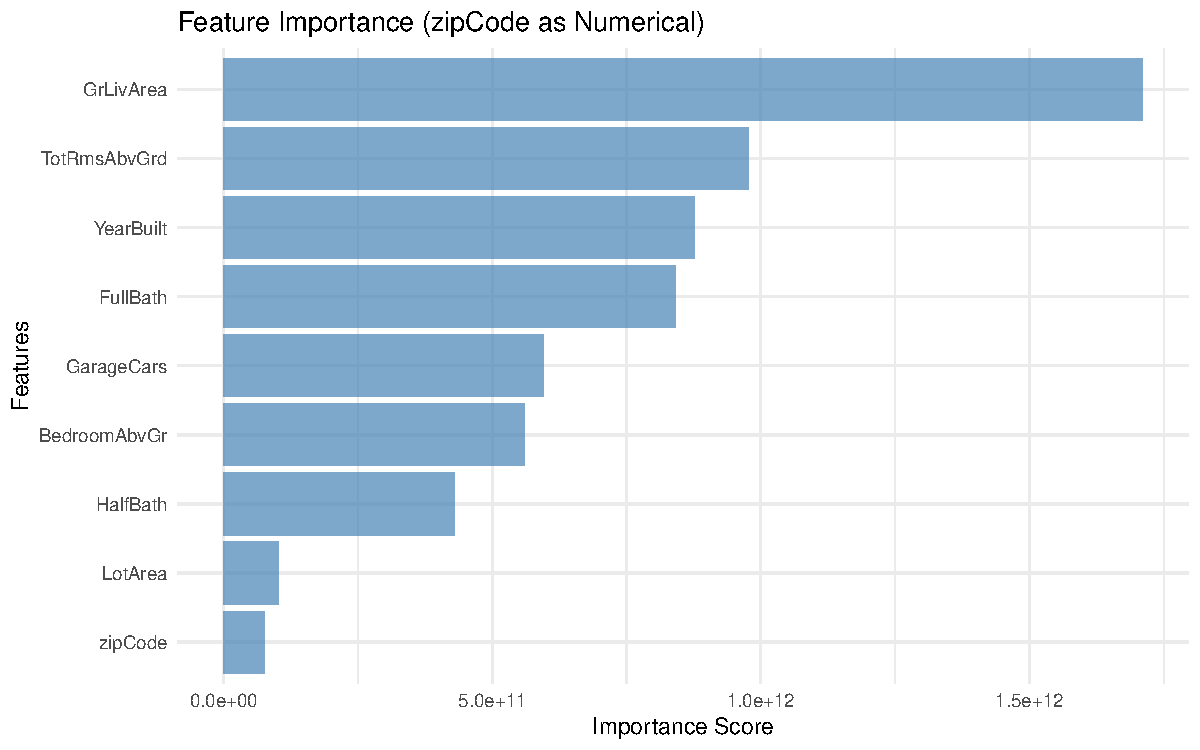
\includegraphics[keepaspectratio]{index_files/figure-pdf/importance-plot-r-1.pdf}}

\subsubsection{Categorical Encoding
Analysis}\label{categorical-encoding-analysis}

\subsubsection{R}\label{r-3}

\begin{Shaded}
\begin{Highlighting}[]
\CommentTok{\# Convert zipCode to factor (categorical)}
\NormalTok{model\_data\_cat }\OtherTok{\textless{}{-}}\NormalTok{ model\_data }\SpecialCharTok{\%\textgreater{}\%}
  \FunctionTok{mutate}\NormalTok{(}\AttributeTok{zipCode =} \FunctionTok{as.factor}\NormalTok{(zipCode))}

\CommentTok{\# Split data}
\FunctionTok{set.seed}\NormalTok{(}\DecValTok{123}\NormalTok{)}
\NormalTok{train\_indices\_cat }\OtherTok{\textless{}{-}} \FunctionTok{sample}\NormalTok{(}\DecValTok{1}\SpecialCharTok{:}\FunctionTok{nrow}\NormalTok{(model\_data\_cat), }\FloatTok{0.8} \SpecialCharTok{*} \FunctionTok{nrow}\NormalTok{(model\_data\_cat))}
\NormalTok{train\_data\_cat }\OtherTok{\textless{}{-}}\NormalTok{ model\_data\_cat[train\_indices\_cat, ]}
\NormalTok{test\_data\_cat }\OtherTok{\textless{}{-}}\NormalTok{ model\_data\_cat[}\SpecialCharTok{{-}}\NormalTok{train\_indices\_cat, ]}

\CommentTok{\# Build decision tree with categorical zipCode}
\NormalTok{tree\_model\_cat }\OtherTok{\textless{}{-}} \FunctionTok{rpart}\NormalTok{(SalePrice }\SpecialCharTok{\textasciitilde{}}\NormalTok{ ., }
                        \AttributeTok{data =}\NormalTok{ train\_data\_cat,}
                        \AttributeTok{method =} \StringTok{"anova"}\NormalTok{,}
                        \AttributeTok{control =} \FunctionTok{rpart.control}\NormalTok{(}\AttributeTok{maxdepth =} \DecValTok{3}\NormalTok{, }
                                              \AttributeTok{minsplit =} \DecValTok{20}\NormalTok{, }
                                              \AttributeTok{minbucket =} \DecValTok{10}\NormalTok{))}

\CommentTok{\# Feature importance with categorical zipCode}
\NormalTok{importance\_cat }\OtherTok{\textless{}{-}} \FunctionTok{data.frame}\NormalTok{(}
  \AttributeTok{Feature =} \FunctionTok{names}\NormalTok{(tree\_model\_cat}\SpecialCharTok{$}\NormalTok{variable.importance),}
  \AttributeTok{Importance =} \FunctionTok{as.numeric}\NormalTok{(tree\_model\_cat}\SpecialCharTok{$}\NormalTok{variable.importance)}
\NormalTok{) }\SpecialCharTok{\%\textgreater{}\%}
  \FunctionTok{arrange}\NormalTok{(}\FunctionTok{desc}\NormalTok{(Importance)) }\SpecialCharTok{\%\textgreater{}\%}
  \FunctionTok{mutate}\NormalTok{(}\AttributeTok{Importance\_Percent =} \FunctionTok{round}\NormalTok{(Importance }\SpecialCharTok{/} \FunctionTok{sum}\NormalTok{(Importance) }\SpecialCharTok{*} \DecValTok{100}\NormalTok{, }\DecValTok{2}\NormalTok{))}

\CommentTok{\# Check if zipCode appears in tree}
\NormalTok{zipcode\_in\_tree }\OtherTok{\textless{}{-}} \StringTok{"zipCode"} \SpecialCharTok{\%in\%} \FunctionTok{names}\NormalTok{(tree\_model\_cat}\SpecialCharTok{$}\NormalTok{variable.importance)}
\ControlFlowTok{if}\NormalTok{(zipcode\_in\_tree) \{}
\NormalTok{  zipcode\_rank\_cat }\OtherTok{\textless{}{-}} \FunctionTok{which}\NormalTok{(importance\_cat}\SpecialCharTok{$}\NormalTok{Feature }\SpecialCharTok{==} \StringTok{"zipCode"}\NormalTok{)}
\NormalTok{\}}
\end{Highlighting}
\end{Shaded}

\subsubsection{Tree Visualization: Categorical
zipCode}\label{tree-visualization-categorical-zipcode}

\subsubsection{R}\label{r-4}

\begin{Shaded}
\begin{Highlighting}[]
\CommentTok{\# Visualize tree with categorical zipCode}
\ControlFlowTok{if}\NormalTok{ (}\FunctionTok{require}\NormalTok{(rpart.plot, }\AttributeTok{quietly =} \ConstantTok{TRUE}\NormalTok{)) \{}
  \FunctionTok{rpart.plot}\NormalTok{(tree\_model\_cat, }
             \AttributeTok{type =} \DecValTok{2}\NormalTok{,}
             \AttributeTok{extra =} \DecValTok{101}\NormalTok{,}
             \AttributeTok{fallen.leaves =} \ConstantTok{TRUE}\NormalTok{,}
             \AttributeTok{digits =} \DecValTok{0}\NormalTok{,}
             \AttributeTok{cex =} \FloatTok{0.8}\NormalTok{,}
             \AttributeTok{main =} \StringTok{"Decision Tree (zipCode as Categorical)"}\NormalTok{)}
\NormalTok{\} }\ControlFlowTok{else}\NormalTok{ \{}
  \FunctionTok{plot}\NormalTok{(tree\_model\_cat, }\AttributeTok{uniform =} \ConstantTok{TRUE}\NormalTok{, }\AttributeTok{main =} \StringTok{"Decision Tree (zipCode as Categorical)"}\NormalTok{)}
  \FunctionTok{text}\NormalTok{(tree\_model\_cat, }\AttributeTok{use.n =} \ConstantTok{TRUE}\NormalTok{, }\AttributeTok{all =} \ConstantTok{TRUE}\NormalTok{, }\AttributeTok{cex =} \FloatTok{0.8}\NormalTok{)}
\NormalTok{\}}
\end{Highlighting}
\end{Shaded}

\pandocbounded{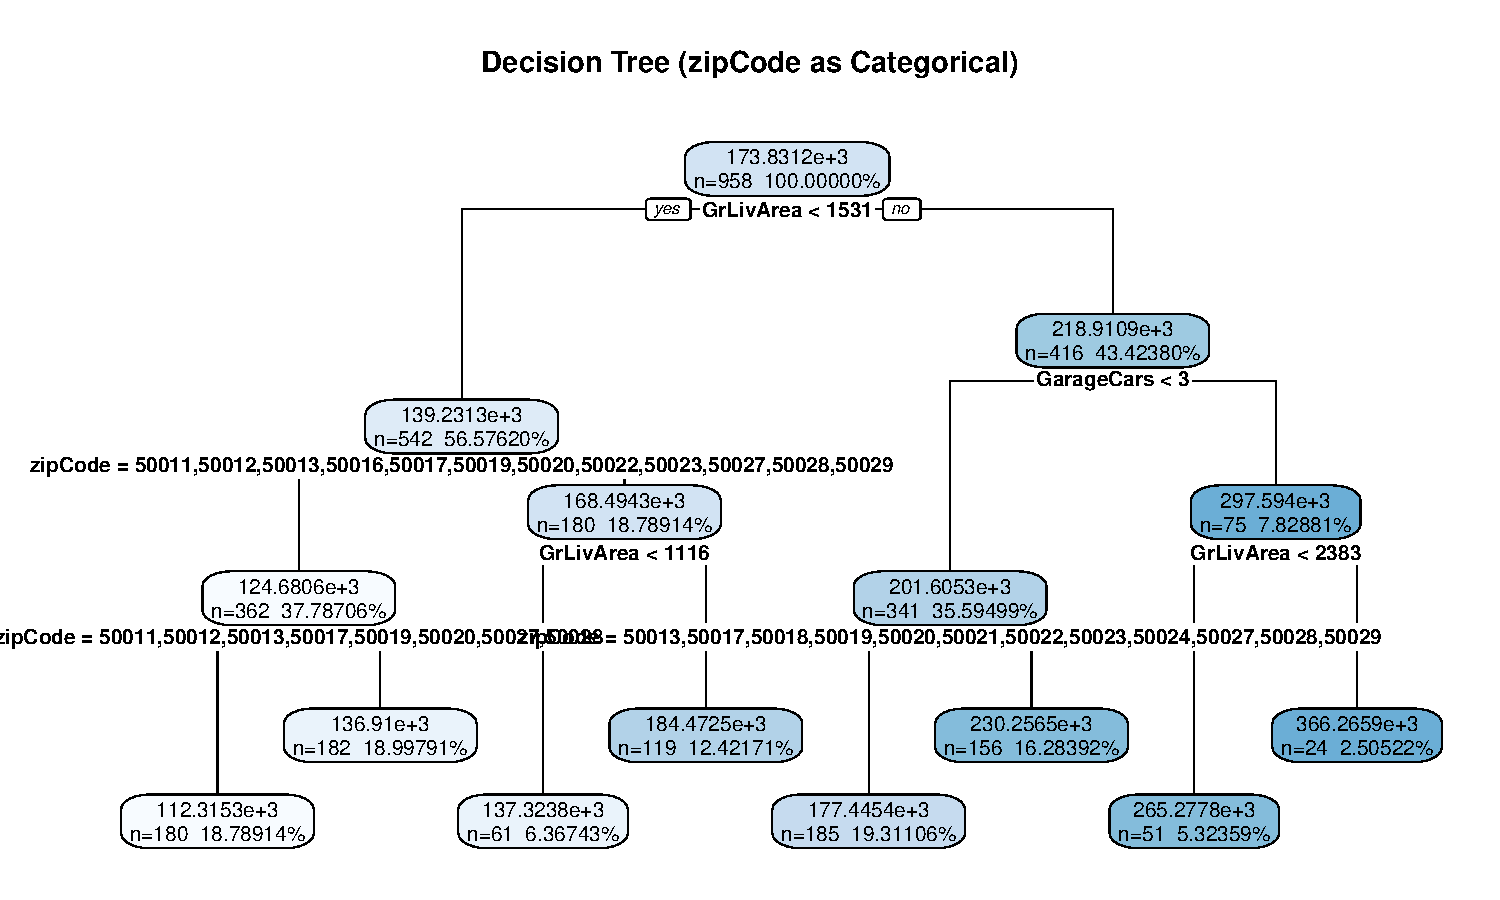
\includegraphics[keepaspectratio]{index_files/figure-pdf/visualize-tree-cat-r-1.pdf}}

\subsubsection{Feature Importance: Categorical
zipCode}\label{feature-importance-categorical-zipcode}

\subsubsection{R}\label{r-5}

\pandocbounded{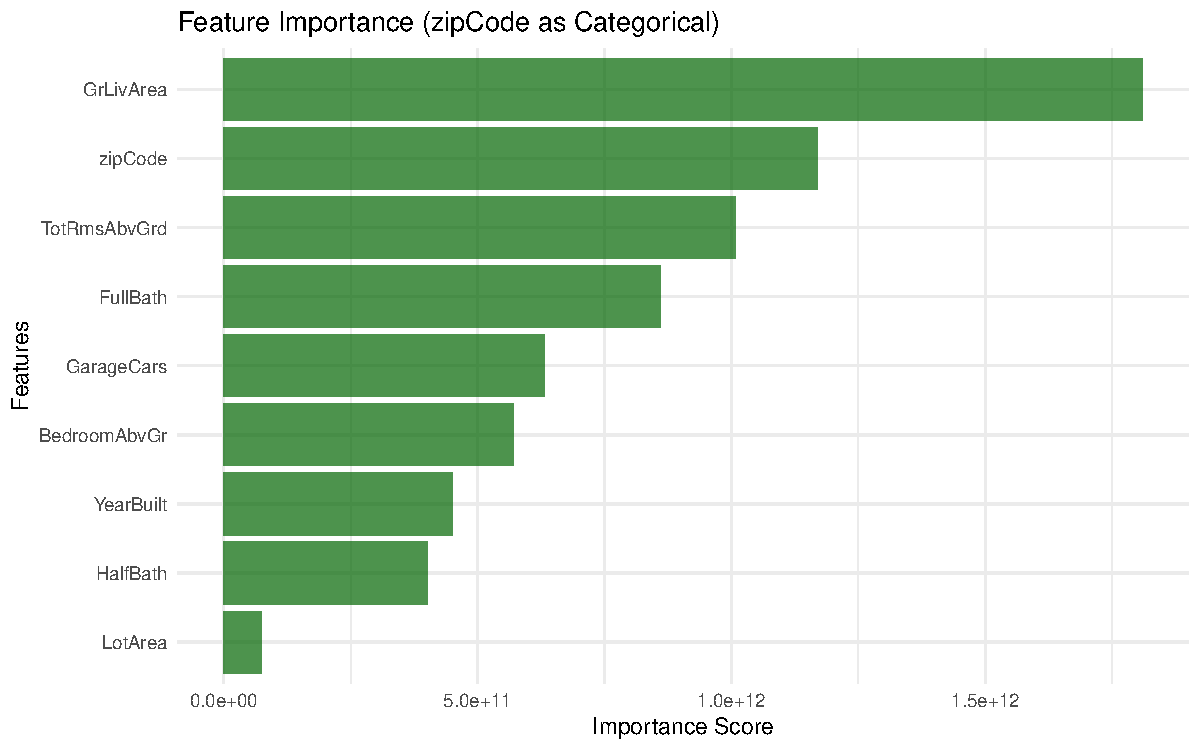
\includegraphics[keepaspectratio]{index_files/figure-pdf/importance-plot-cat-r-1.pdf}}

\subsection{Discussion Questions for
Challenge}\label{discussion-questions-for-challenge}

\textbf{Narrative}

\begin{enumerate}
\def\labelenumi{\arabic{enumi}.}
\item
  Zip codes are not averaged, added, or used in any arithmetic
  sequences. They should be modeled categorically since they refer to a
  town, and not a number of some kind. In the sense of real estate, each
  zip code should be categorical, which allows them to be intercepts.
  Zip codes capture areas and represent the housing prices in that
  location. It will influence price analysis in a categorical way.
\item
  R has more sensible splits because of packages like randomforest. This
  helps to pass variables directly in groupings that are produced by the
  algorithm itself. In contrast, Python uses packages like scikit-learn
  that requires you to encode categorical variables. If you do not
  speficfy beforehand, the package assumes all inputs are numeric. The
  rpart ``splits a numeric matrix describing the splits: \ldots{} the
  row label is the name of the split variable \ldots{} For a factor
  \ldots{} the index column contains the row number of the csplit
  matrix.'' (Therneau 2025) R give the freedom to the algorithm to group
  ZIP codes as categorical values based on outcome distribution. Having
  to do a one-hot encode will create a dilution of feature importance,
  since it will be spread into many dummy columns.
\end{enumerate}




\end{document}
